\documentclass[border=10pt]{standalone}

\usepackage{tikz}
\usepackage{tikzsymbols}
\usetikzlibrary{calc,patterns,shapes.geometric}

\def\centerarc[#1](#2)(#3:#4:#5){\draw[#1] ($(#2)+({#5*cos(#3)},{#5*sin(#3)})$) arc (#3:#4:#5);}

\begin{document}
	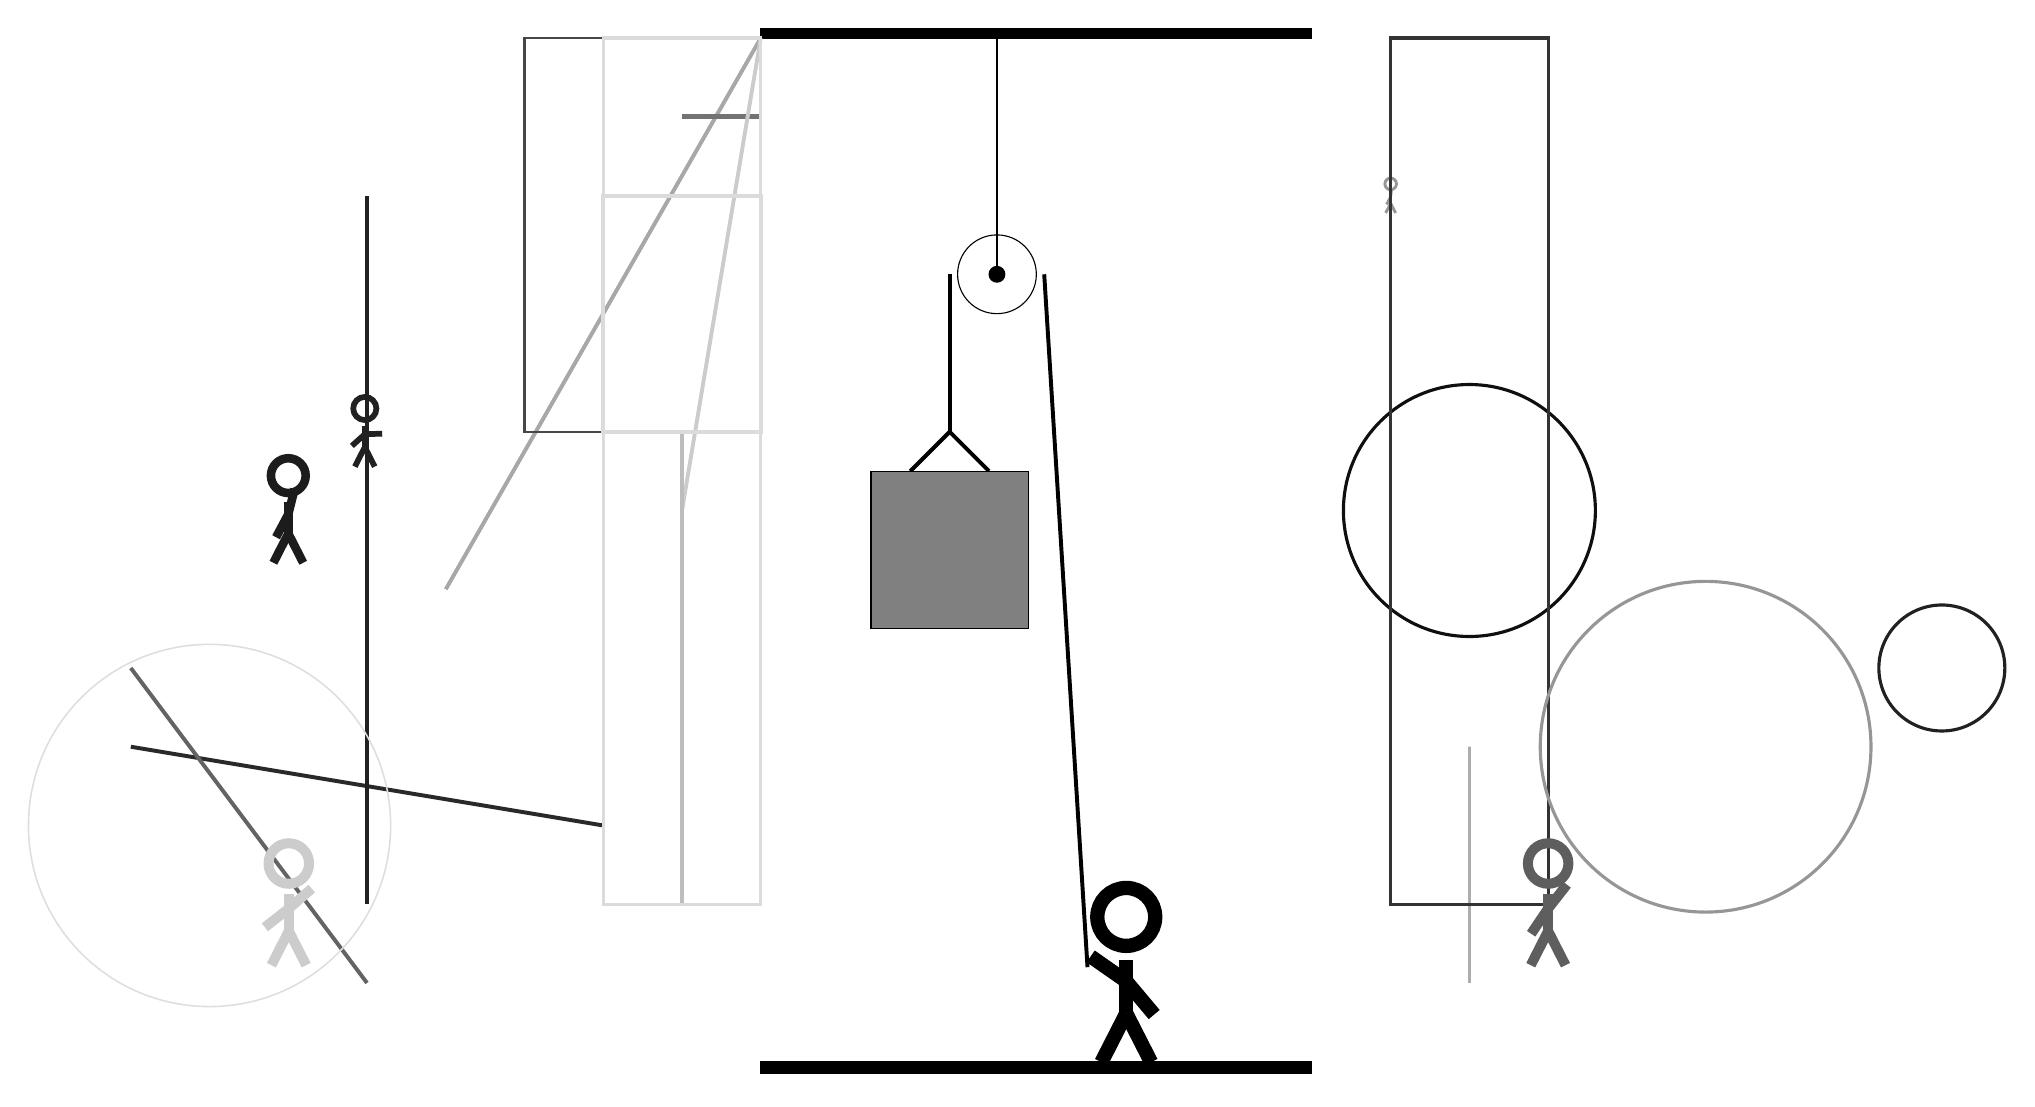
\begin{tikzpicture}
		%%%%% START %%%%%
		
		\draw[fill=black] (-2, 10) rectangle (5, 10.125);
		
		\draw (1, 7) circle (0.5);
		\draw[fill=black] (1, 7) circle (0.1);
		\draw (1, 10) -- (1, 7);
		
		\draw[line width=0.5mm, color=black!84](-4, 0) -- (-10, 1);
		
		\draw[line width=0.3mm, color=black!32] (7, -2) rectangle (7, 1);
		\draw[line width=0.5mm, color=black!34](-6, 3) -- (-2, 10);
		\draw [line width=0.4mm, color=black!94](7, 4) circle (1.6);
		
		\draw[line width=0.6mm, color=black!55] (-3, 9) rectangle (-2, 9);
		
		\node[line width=0.2mm, color=black!41] at (6, 8) {\Strichmaxerl[2][62][84]};
		
		\draw[line width=0.3mm, color=black!72] (-4, 5) rectangle (-5, 10);
		\draw[line width=0.5mm, color=black!61](-7, -2) -- (-10, 2);
		\draw[line width=0.4mm, color=black!80] (6, 10) rectangle (8, -1);
		\draw[line width=0.5mm, color=black!20](-2, 10) -- (-3, 4);
		\node[line width=0.4mm, color=black!89] at (-8, 4) {\Strichmaxerl[6][62][76]};
		\draw[line width=0.5mm, color=black!26](-3, -1) -- (-3, 5);
		\draw[line width=0.5mm, color=black!87](-7, -1) -- (-7, 8);
		
		\draw [line width=0.4mm, color=black!87](13, 2) circle (0.8);
		\node[line width=0.7mm, color=black!63] at (8, -1) {\Strichmaxerl[7][56][52]};
		\draw [line width=0.4mm, color=black!41](10, 1) circle (2.1);
		
		\node[line width=0.5mm, color=black!20] at (-8, -1) {\Strichmaxerl[7][38][41]};
		\draw [line width=0.2mm, color=black!13](-9, 0) circle (2.3);
		\node[line width=0.5mm, color=black!87] at (-7, 5) {\Strichmaxerl[4][42][2]};
		\draw[line width=0.5mm, color=black!14] (-2, 5) rectangle (-4, 8);
		\draw[line width=0.4mm, color=black!14] (-4, -1) rectangle (-2, 10);
		
		\draw[line width=0.5mm] (-0.1, 4.5) -- (0.4, 5.0) -- (0.9, 4.5);
		\draw[fill=black!50] (-0.6, 4.5) rectangle (1.4, 2.5);
		
		\draw[line width=0.5mm] (0.4, 7) -- (0.4, 5.0);
		\centerarc[line width=0.5mm](1, 7)(0:180:0.6);
		\draw[line width=0.5mm](1.6, 7) -- (2.15, -1.8);
		
		\node at (2.6, -1.9) {\Strichmaxerl[10][-35][-50]};
		
		\draw[fill=black] (-2, -3) rectangle (5, -3.15);
		
		%%%%% END %%%%%
	\end{tikzpicture}
\end{document}